% Software License Agreement
%
% Author    Tony Baltovski <tbaltovski@clearpathrobotics.com>
% Copyright (c) 2020, Clearpath Robotics, Inc., All rights reserved.
%
% Redistribution and use in source and binary forms, with or without modification, is
% not permitted without the express permission of Clearpath Robotics.

\documentclass[]{clearpath-latex/clearpath-manual}
\graphicspath{{gen/}}
\usepackage{float}
\usepackage{fancyhdr}
\pagestyle{fancyplain}
\lfoot{Rev. 1.1.0}
\rfoot{Dingo}
\lhead{}
\chead{}
\rhead{}
\renewcommand{\headrulewidth}{0pt}





\begin{document}

\manualcover{cover-page.pdf}
\tableofcontents

\section{Introduction}

Dingo is a lightweight and easy-to-use unmanned indoor ground vehicle for ROS
Melodic, presented by Clearpath Robotics.

Dingo includes a standard internal PC, as well as basic IMU. Standard
perception modules are available, including URDF and simulator integration, as well as demonstration applications.

There are two Dingo variants:
\begin{itemize}[nolistsep]
	\item Dingo-D: Uses differential drive and has two module bays, one of which must be a battery module; the second module is typically a computer module.
	\item Dingo-O: Uses omnidirectional drive and has four module bays, at least two of which are typically battery modules; the other modules may be computer modules or serve as expansion for other custom hardware.
\end{itemize}

Please inquire with Clearpath Robotics for details. See \nameref{contact} on page
\pageref{contact} for contact information.

\subsection{What's Included}

Contained in your Dingo shipment are the following items:

\begin{itemize}[nolistsep]
  \item Dingo UGV (Dingo-D or Dingo-O variant)
  \item One or more 12V sealed lead acid (SLA) or 14.4V Lithium-ion batteries
  \item One or more 110/220V universal chargers for your batteries
  \item One Sony PS4 Bluetooth controller
  \item One Dingo User Manual
\end{itemize}

If you elected to purchase standard payload modules or custom integration services with
Dingo, then additional equipment will be included per your specific configuration, plus
further documentation as required.

\subsection{Hardware Overview}

Dingo's external features include the mounting pattern on the top trough cover, \SI{98.4}{\mm} diameter
wheels (Dingo-D) or \SI{101.6}{\mm} diameter mechanum wheels (Dingo-O), human machine interface panel (HMI), top (yellow) fairings, and side access panels. The exteriors of Dingo-D and Dingo-O are shown in \autoref{ext-d} and \autoref{ext-o} respectively.

\begin{figure}[pt]
  \centering
  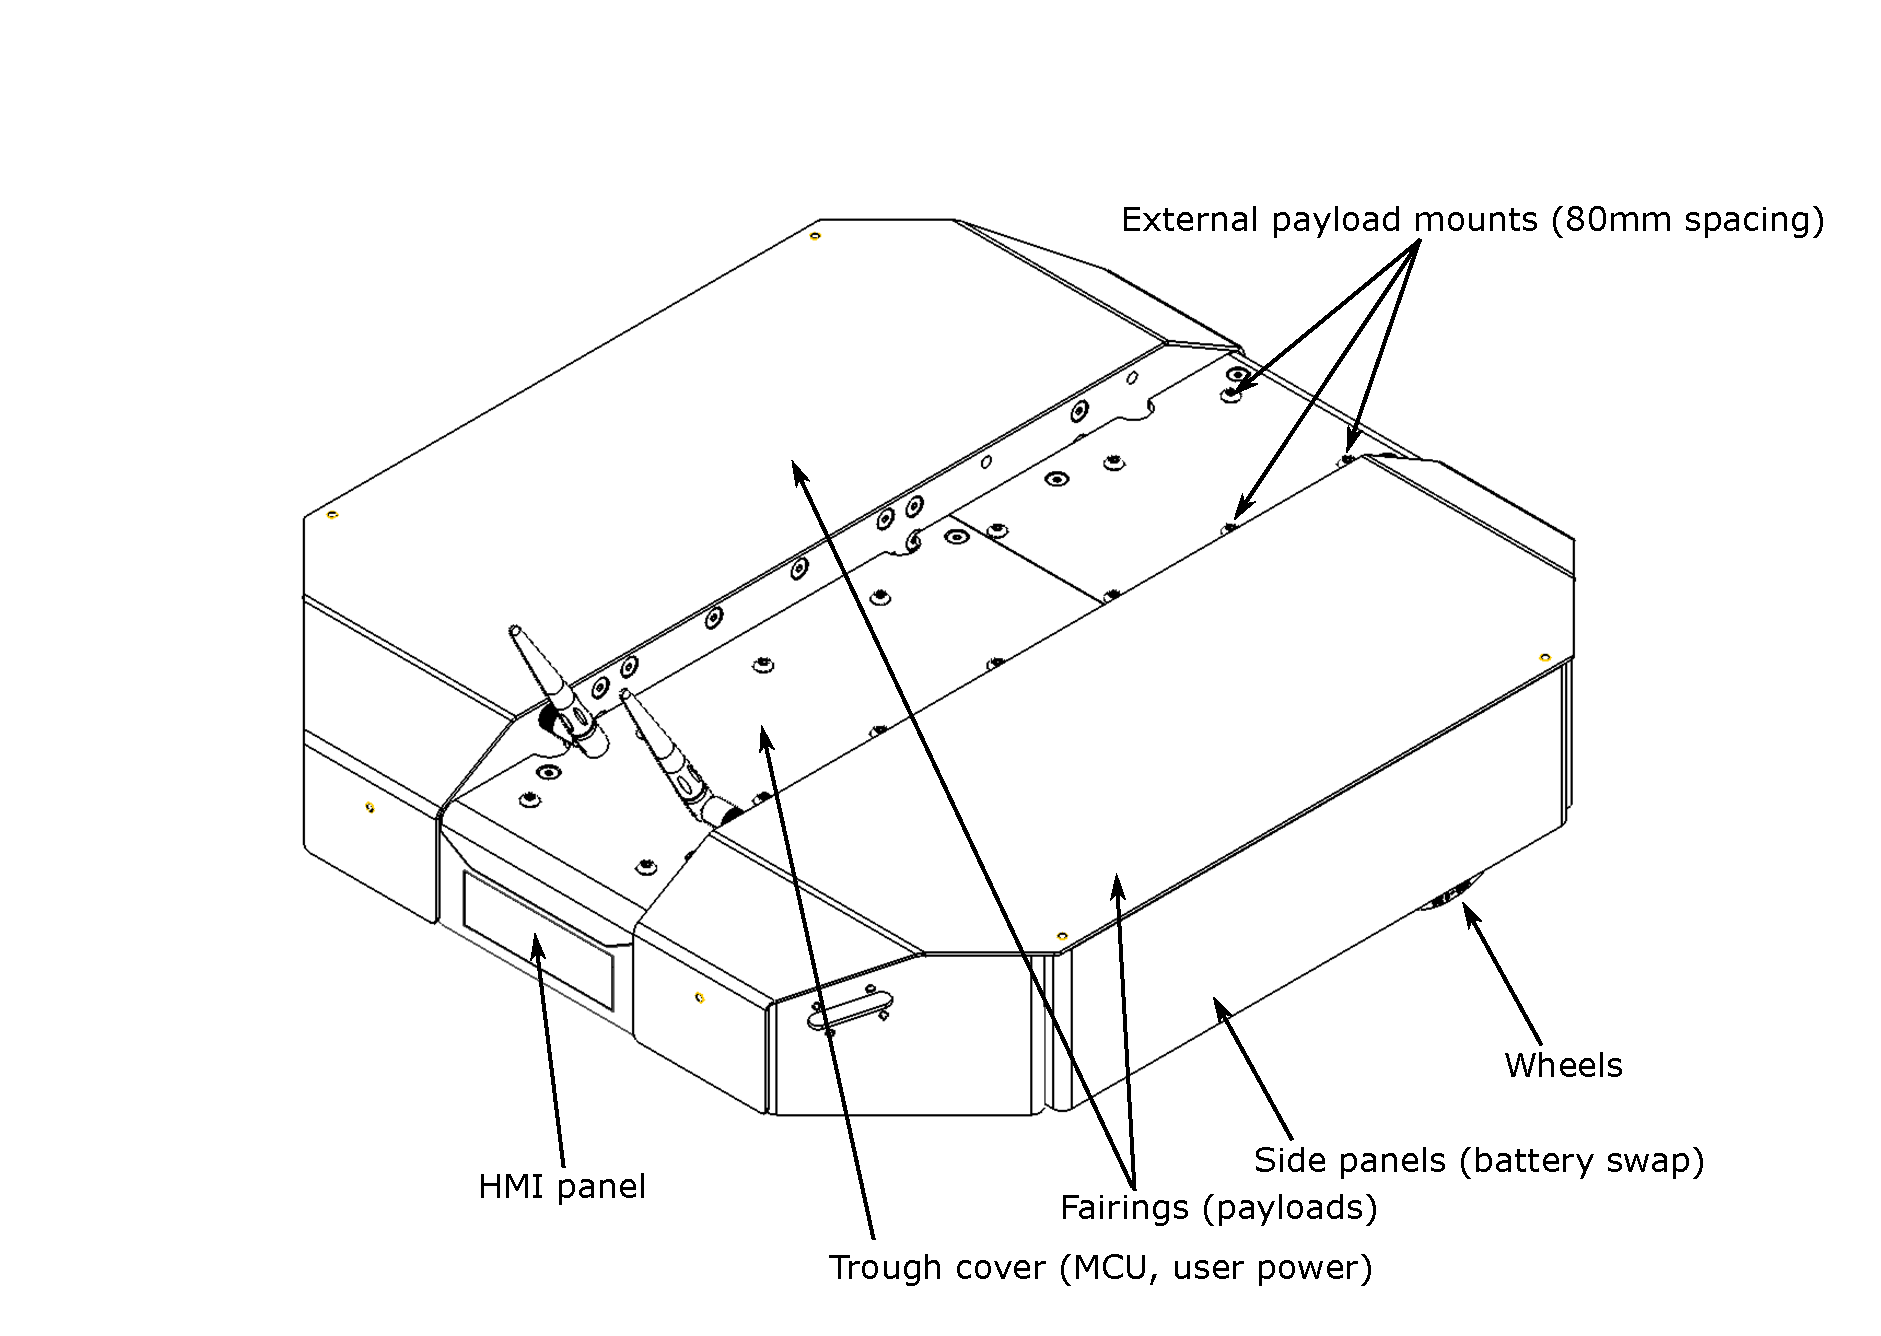
\includegraphics[width=12.0cm]{dingo-d-ext.pdf}
  \caption{Dingo-D exterior}
  \label{ext-d}
\end{figure}

\begin{figure}[pt]
  \centering
  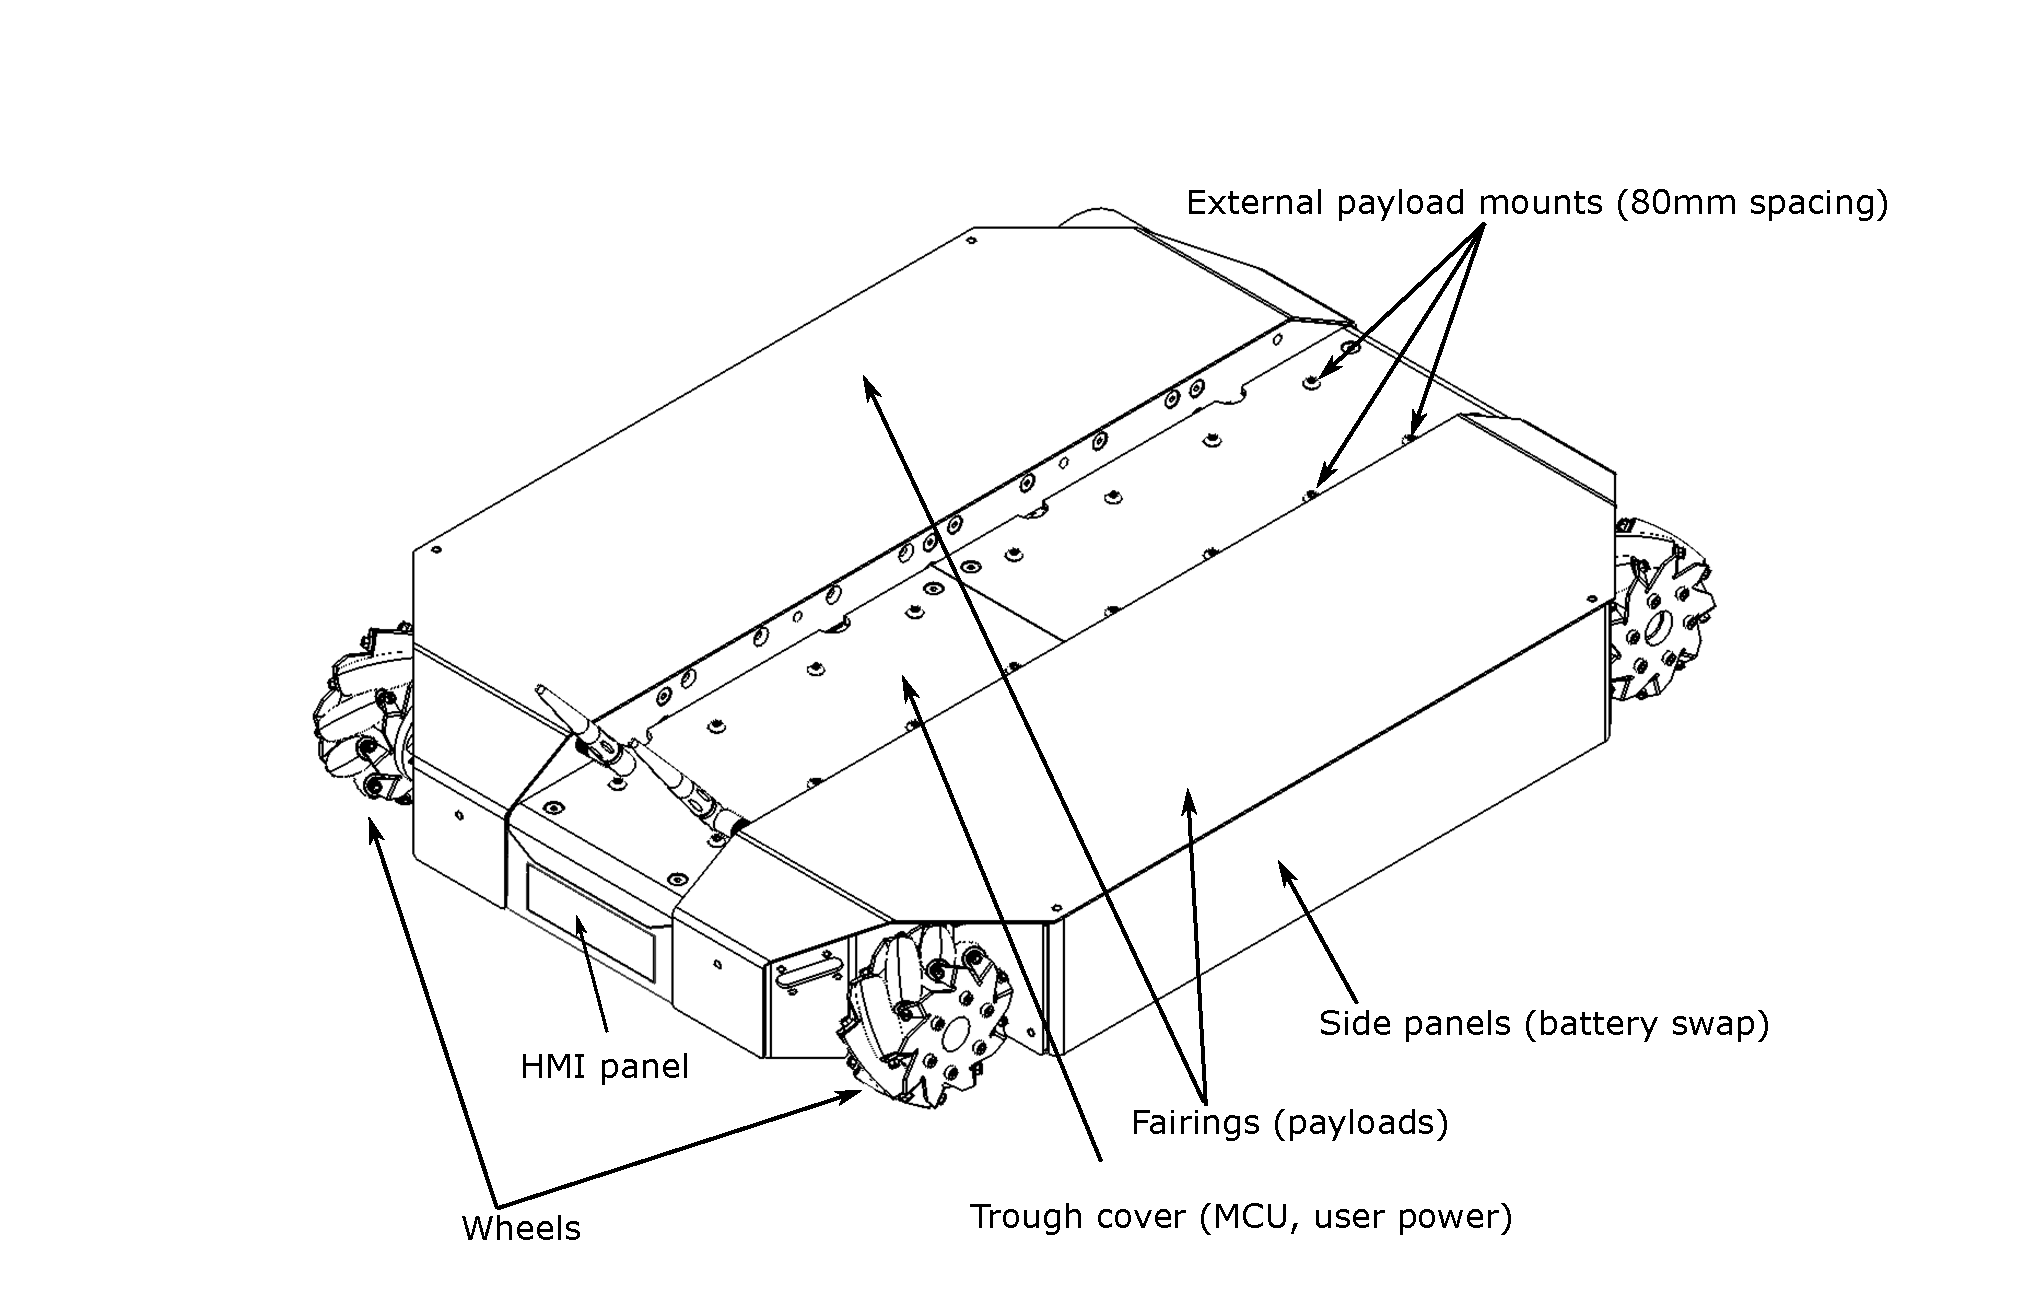
\includegraphics[width=12.0cm]{dingo-o-ext.pdf}
  \caption{Dingo-O exterior}
  \label{ext-o}
\end{figure}

The HMI panel is shown in
\autoref{hmi}, and includes from left: motor stop button, comms indictor, wifi indicator, battery
indicator, and system power button.

\begin{figure}[ht]
  \centering
  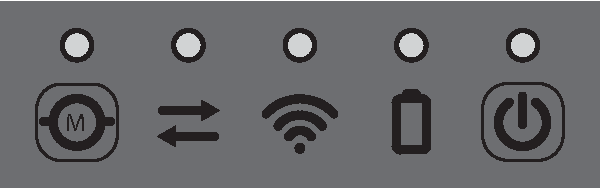
\includegraphics[width=8.0cm]{hmi.pdf}
  \caption{HMI panel.}
  \label{hmi}
\end{figure}

To access Dingo's payload modules (computers or batteries), simply slide and remove the top (yellow) fairings. To access Dingo's MCU PCBA (for user power), remove the four M5 flathead screws from the top trough cover, and then remove the trough cover.

The interior of the Dingo-D is shown in \autoref{int-d} and the interior of Dingo-O is shown in \autoref{int-o} along with example payload modules.

\begin{figure}[pt]
  \centering
  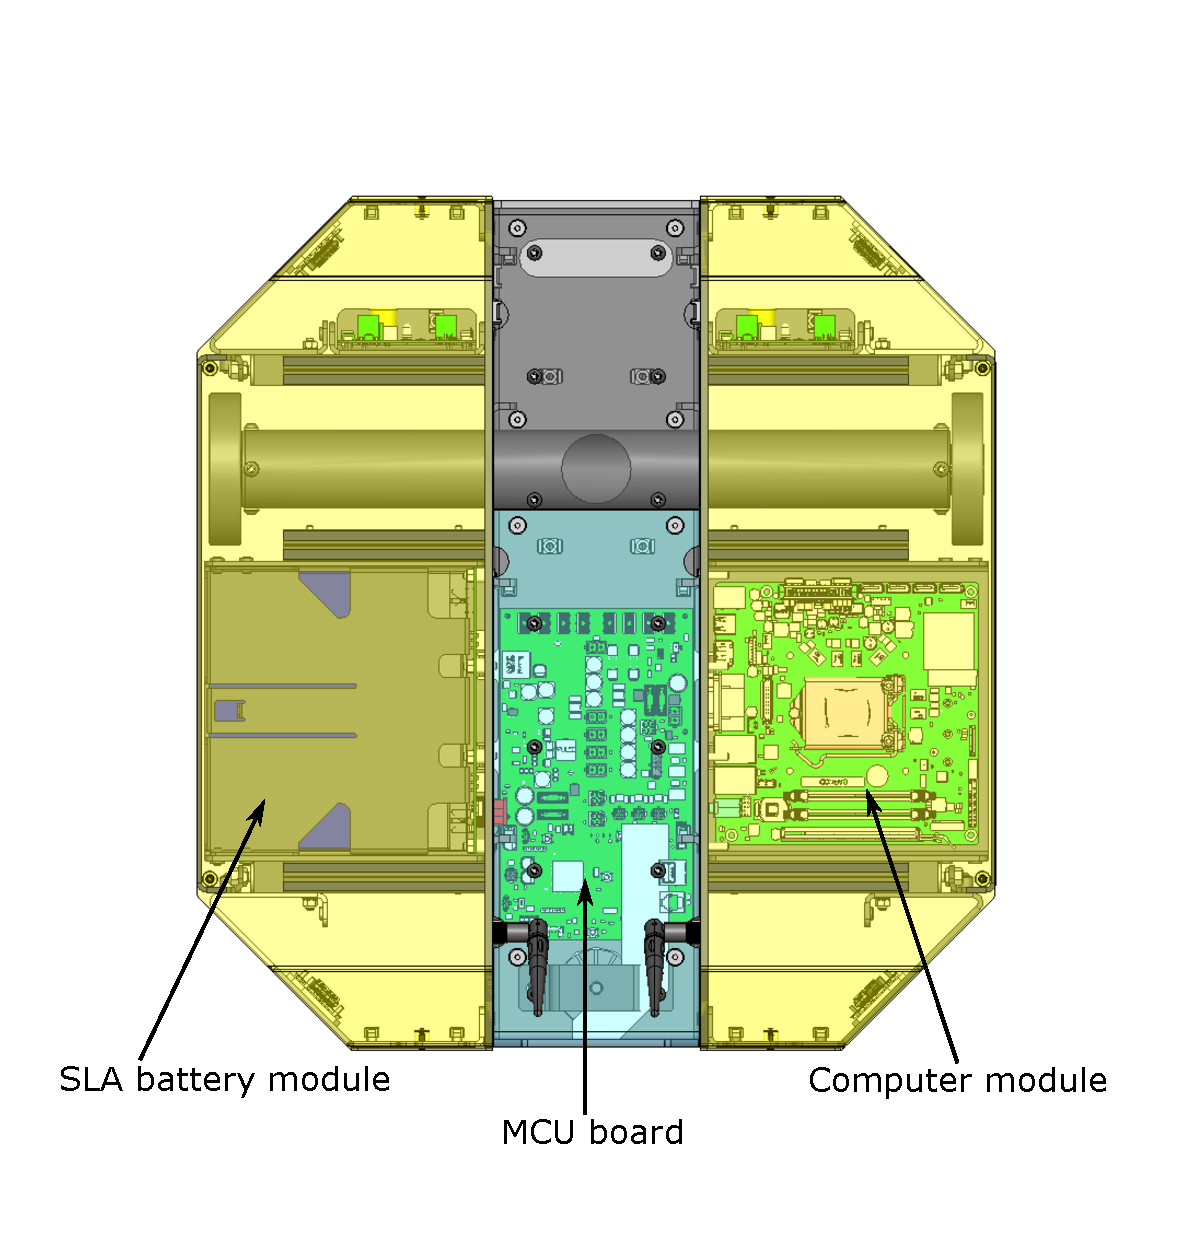
\includegraphics[width=9.0cm]{dingo-d-int.pdf}
  \caption{Area inside Dingo-D, with example modules}
  \label{int-d}
\end{figure}

\begin{figure}[pt]
  \centering
  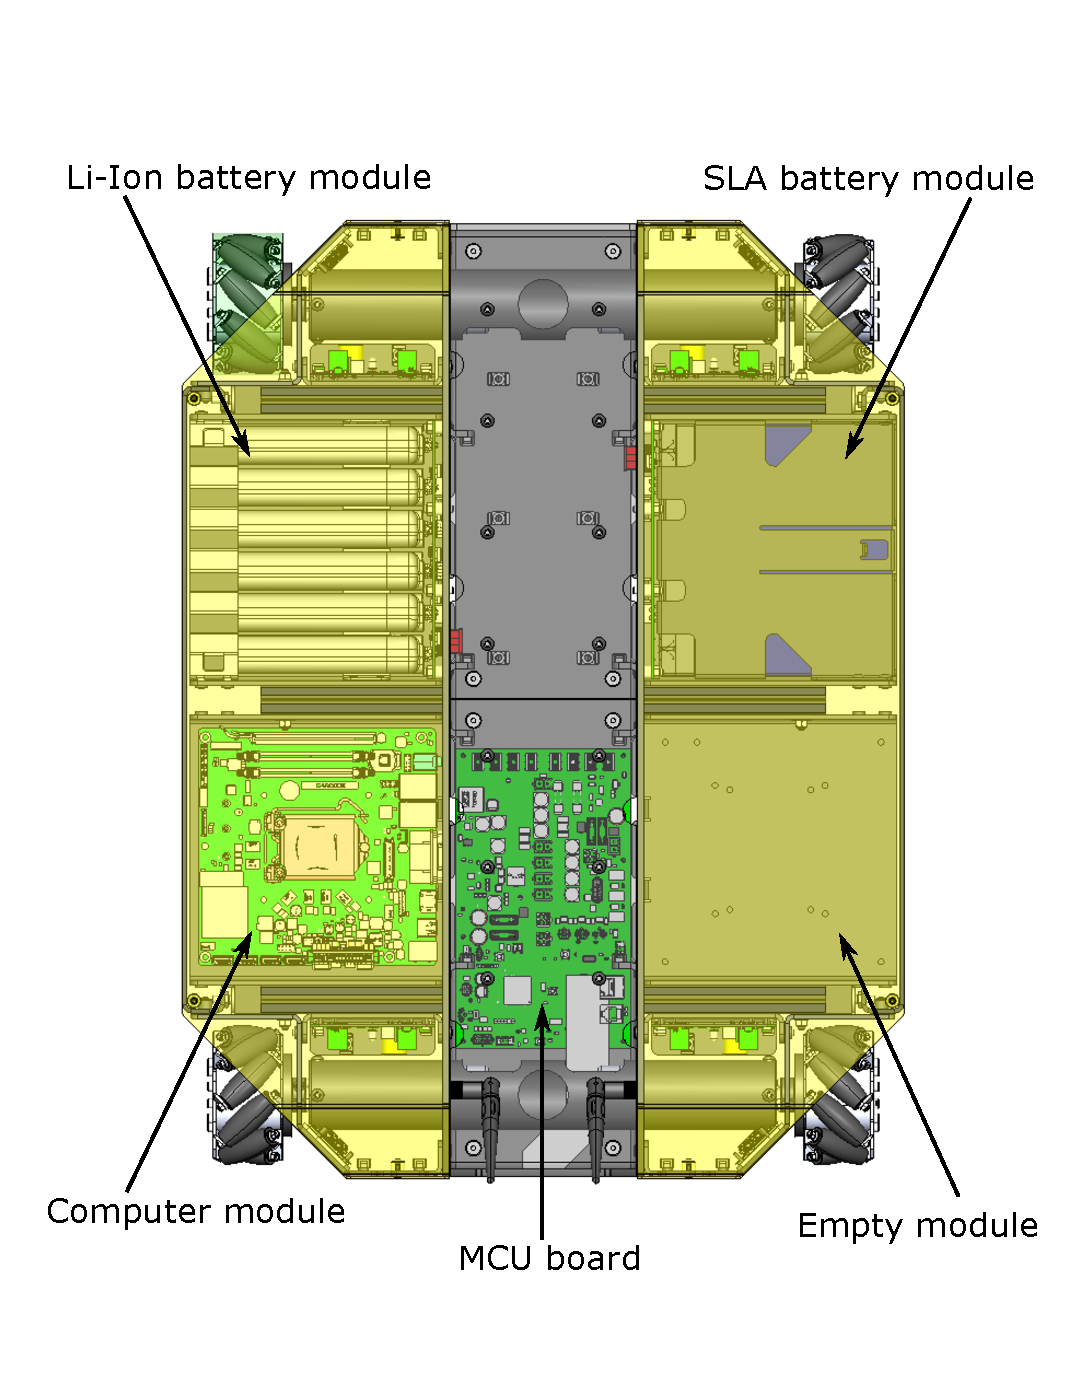
\includegraphics[width=9.0cm]{dingo-o-int.pdf}
  \caption{Area inside Dingo-O, with example modules}
  \label{int-o}
\end{figure}

Dingo-D will contain one battery module (Sealed Lead Acid or Lithium Ion) and Dingo-O will contain one or more battery modules. Batteries can be installed and removed by removing the corresponding side access panel and sliding the battery in or out as needed.

Dingo does provide an optional shore power connection to allow the system to be powered without requiring batteries to be present. Note that when shore power is connected, the motors are disabled and it is not possible to drive the Dingo; however, all other electronics (computers, sensors, etc) will remain enabled.

\subsection{System Architecture}

Like many ROS robots, Dingo is built around an x86 PC running Ubuntu, paired with a
32-bit MCU. The MCU handles I/O, power supply monitoring, and motor control, as well as
supplying data from the integrated IMU. The communication channel
between the MCU and PC is a Gigabit Ethernet connection.

The key topics which comprise Dingo's ROS API are given in \autoref{table:rosapi}.

\bgroup
\begin{table}[htp]
\begin{tabular}{  l  l  p{7cm} }
\hline
Topic & Message Type & Purpose \\ \hline

\lstinline!/cmd_vel! & \lstinline!geometry_msgs/Twist! &
Input to Dingo's kinematic controller. Publish here to make Dingo go. \\ \hline
\lstinline!/odometry/filtered! & \lstinline!nav_msgs/Odometry! &
Published by \lstinline!robot_localization!, a filtered localization estimate based
on wheel odometry (encoders), and integrated IMU. \\ \hline

\lstinline!/imu/data! & \lstinline!sensor_msgs/IMU! &
Published by \lstinline!imu_filter_madgwick!, an orientation estimate based on Dingo's
internal IMU unit. \\ \hline

\lstinline!/mcu/status! & \lstinline!dingo_msgs/Status! &
Low-frequency status data for Dingo's systems. This information is republished in human
readable form on the \lstinline!diagnostics! topic and is best consumed with the Robot
Monitor. \\ \hline
\end{tabular}
\caption{Dingo ROS API Topics}
\label{table:rosapi}
\end{table}
\egroup

\section{Getting Started}

The first step is to power up your Dingo and have some fun driving it around! If you've
just unpacked Dingo from its packaging, you may need to open it up and connect the
battery.

Press the power button \raisebox{-0.4em}{
\includegraphics[width=0.5cm]{icon-power.pdf}} on
Dingo's HMI panel. The LEDs should show a test pattern, after which you will wait about 30
seconds for the internal PC to finish booting up.

When the comms LED (\raisebox{-0.4em}{
\includegraphics[width=0.5cm]{icon-comms.pdf}}) is
green, this signals that the PC is finished booting up, and that the PC and MCU are in
communication. At this point,
press the PS button on the Sony Bluetooth controller to sync the controller to Dingo. Once
the blue LED on the top of the controller goes solid, you're paired and ready to drive. Hold the L1 trigger
button (deadman switch), and push the left thumbstick forward to drive the Dingo. For full speed mode, hold the R1 trigger.  See \autoref{ps4layout} for the Sony PS4 controls layout.

\begin{figure}[H]
  \centering
  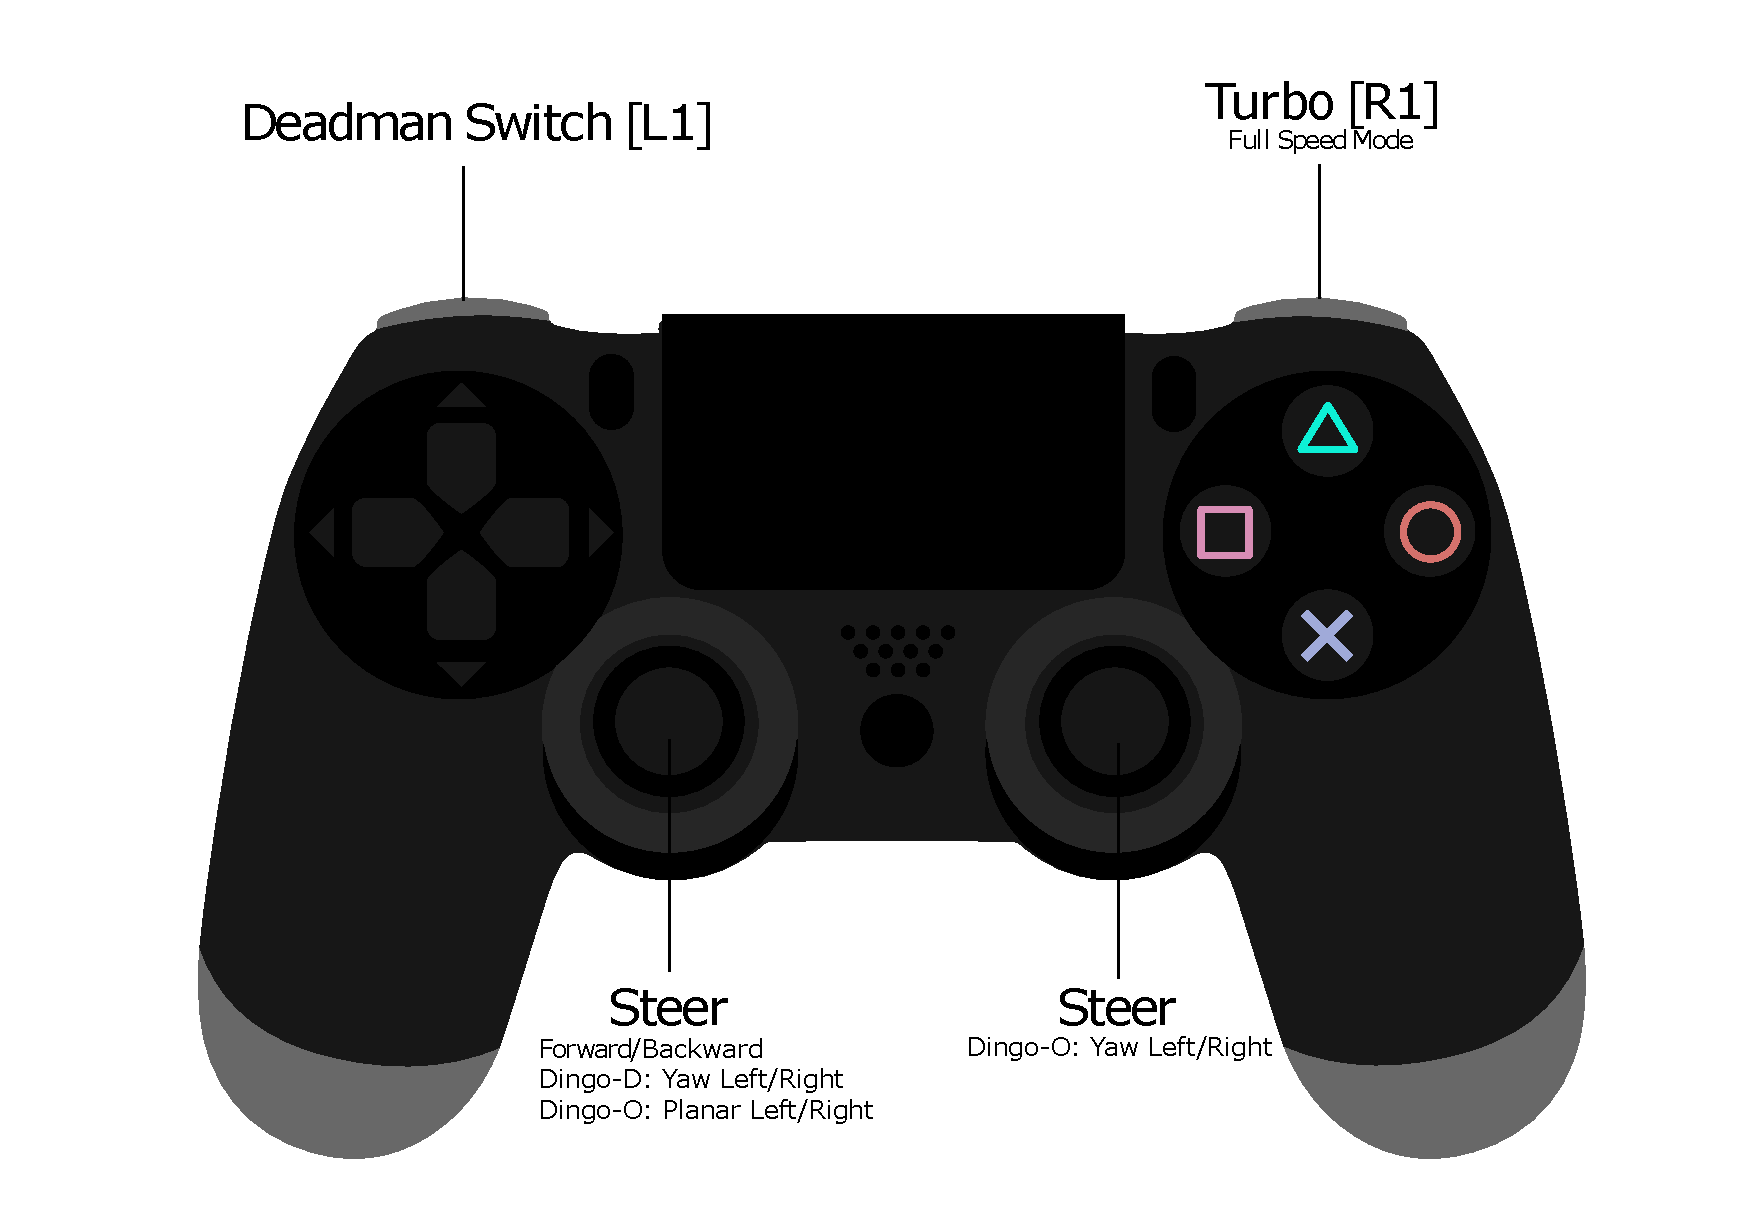
\includegraphics[width=0.75\linewidth]{dingo-sony-ps4-controller-labelled.pdf}
  \caption{PS4 Controls Layout}
  \label{ps4layout}
\end{figure}


If you're not seeing any action, check \nameref{trouble} on page \pageref{trouble} to
get in touch with support.

\subsection{Wireless Access}

To get Dingo connected to your local wifi, you must first access the internal computer
using a wired connection. Open the chassis, lower the computer tray, and connect to the network port
labeled \lstinline{STATIC} with a standard ethernet cable.

\subsubsection{Static IP Configuration}

Set your laptop's ethernet port to a static IP such as \lstinline{192.168.131.51}.  To do this in Ubuntu, follow the steps below:
\begin{enumerate}
  \item Click on the Wifi icon in the upper-right corner of your screen, and select \textbf{Edit Connections}
  \item In the \textbf{Network Connections} window, under \textbf{Ethernet}, select your wired connection and then click \textbf{Edit}
  \item Select the \textbf{IPv4 Settings} tab and then change the \textbf{Method} to \lstinline{Manual}
  \item Click the \textbf{Add} button to add a new address
  \item Enter a \lstinline{192.168.131.51} as the static IP under the \textbf{Address} column, and enter \lstinline{255.255.255.0} under the \textbf{NetMask} column, and then select \textbf{Save}
\end{enumerate}

\begin{figure}[H]
  \centering
  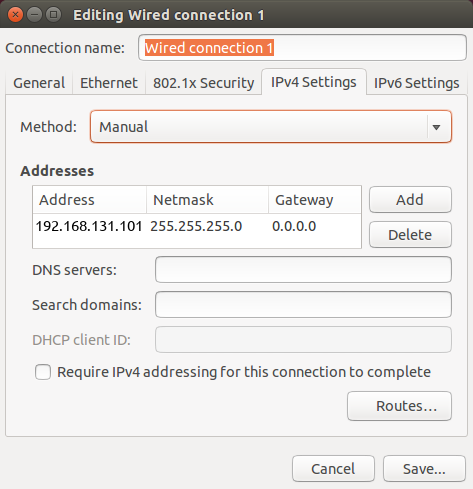
\includegraphics[width=0.5\linewidth]{wired_connection.png}
  \caption{Static IP Configuration}
  \label{staticip}
\end{figure}


\subsubsection{Connect to Dingo via SSH over ethernet}

The next step is to connect to Dingo via SSH.  To do so execute the following in a terminal window:

\begin{lstlisting}
ssh administrator@192.168.131.1
\end{lstlisting}

You will be promoted to enter a password.  The default password is \lstinline{clearpath}.

\subsubsection{Connect Dingo to Wireless Network}

Now that you're connected via SSH over a wired connection, you can setup Dingo to connect to a local wifi network.  To do this, you will use the wireless interface configuration daemon (WICD) - a preinstalled network manager.

In a terminal window, execute the following command:

\begin{lstlisting}
wicd-curses
\end{lstlisting}

You should see a browsable list of networks which the robot has detected. Use arrow keys to select the one you would like to connect to, and then press the right arrow to configure it. You can enter your network’s password near the bottom of the page, and note that you must select the correct encryption scheme; most modern networks use WPA1/2 Passphrase, so if that’s you, make sure that option is selected. You also likely want to select the option to automatically reconnect to this network, so that Dingo will be there for you on your wireless automatically in the future.

When you’re finished, press \textbf{F10} to save, and then \textbf{C} to connect.  Dingo is now connected to wifi!

While you're still wired to Dingo, you'll need to identify the IP address of Dingo's wireless connection.

In a terminal window, execute:

\begin{lstlisting}
ifconfig
\end{lstlisting}

A list of network connections will be displayed within the terminal.  Locate the wireless network and make note of its IP address. Now that you know Dingo's wireless IP address, you may now exit the ethernet SSH session by executing \lstinline{exit}.

Remove the ethernet cable and close up Dingo.   Now you can SSH into Dingo over the wireless network.  To do so, execute:

\begin{lstlisting}
ssh administrator@<IP_OF_DINGO>
\end{lstlisting}

SSH sessions allow you to control Dingo's internal computer.  You can do various things such as download packages, run updates, add/remove files, transfer files etc.

\subsection{Remote ROS Connectivity}\label{remote}

To use ROS desktop tools, you’ll need your computer to be able to connect to Dingo’s ROS master. This will allow you to run ROS commands like \lstinline{rostopic list}, \lstinline{rostopic echo}, \lstinline{rosnode list}, and others, from a remote PC and the output will reflect the activity on Dingo’s ROS master, rather than on your own machine.  This can be a tricky process, but we’ve tried to make it as simple as possible.

In order for the ROS tools on your computer to talk to Dingo, they need to know two things:

\begin{itemize}[nolistsep]
  \item How to find the ROS master, which is set in the \lstinline{ROS_MASTER_URI} environment variable, and
  \item How processes on the other computer can find your computer, which is the \lstinline{ROS_IP} environment variable.
\end{itemize}

The suggested pattern is to create a file in your home directory called \lstinline{remote-dingo.sh} with the following contents:

\begin{lstlisting}
export ROS_MASTER_URI=http://cpr-dingo-0001:11311  # Dingo's hostname
export ROS_IP=10.25.0.102       # Your laptop's wireless IP address
\end{lstlisting}

If your network doesn’t already resolve Dingo’s hostname to its wireless IP address, you may need to add a corresponding line to your computer’s /etc/hosts file:

\begin{lstlisting}
10.25.0.101 cpr-dingo-0001
\end{lstlisting}

\textbf{NOTE:} You can verify the hostname and IP address of Dingo using the following commands during an SSH session with the onboard PC.

\begin{lstlisting}
hostname
hostname -i
\end{lstlisting}

Then, when you’re ready to communicate remotely with Dingo, you can source that script like so, thus defining those two key environment variables in the present context.

\begin{lstlisting}
source remote-dingo.sh
\end{lstlisting}

To verify that everything is set up propelry, try running a few ROS commands, such as the standard visual ROS tools:

\begin{lstlisting}
roslaunch dingo_viz view_robot.launch
rosrun rqt_robot_monitor rqt_robot_monitor
rosrun rqt_console rqt_console
\end{lstlisting}

If the tools launch, then everything is setup properly.

Please contact Clearpath Support if you need assistance in configuring remote access. For more general details on how ROS works over TCP with multiple machines, please see:

\url{http://wiki.ros.org/ROS/Tutorials/MultipleMachines}.

For help troubleshooting a multiple machines connectivity issue, see:

\url{http://wiki.ros.org/ROS/NetworkSetup}

\newpage\subsection{Dingo Desktop Packages}

To command or observe Dingo from your desktop computer, first set up a basic
ROS installation. See the following page for details:

\url{http://wiki.ros.org/melodic/installation/ubuntu}

When your ROS install is set up, install the Dingo desktop packages:

\begin{lstlisting}
sudo apt-get install ros-melodic-dingo-desktop
\end{lstlisting}

Once your remote access to Dingo's ROS master is configured (see options in \autoref{remote}),
you can launch rviz, the standard ROS robot visualization tool:

\begin{lstlisting}
roslaunch dingo_viz view_robot.launch
\end{lstlisting}

From within rviz, you can use interactive markers to drive Dingo, you can visualize its
published localization estimate, and you can visualize any attached sensors which have been
added to its robot description XML (\lstinline{URDF}).

Additionally from the desktop, you can launch the standard RQT Robot Monitor, which
watches the diagnostic output from Dingo's self-montoring capabilities:

\begin{lstlisting}
rosrun rqt_robot_monitor rqt_robot_monitor
\end{lstlisting}

\section{Apps}

When equipped with a laser scanner as is available in the Gazebo simulation, Dingo works with the
standard ROS navigation stack. See \url{http://wiki.ros.org/dingo_navigation}.


\section{Charging \& Battery Maintenance}

When finished with the Dingo, press and release the power button \raisebox{-0.4em}{
\includegraphics[width=0.5cm]{icon-power.pdf}} to power it off. Then remove the batteries for charging.

Dingo's batteries are charged outside the Dingo using the charger(s) provided.

Alternatively, if you have multiple batteries, you can hot-swap them one at a time. The system will remain operational while hot-swapping as long as there is at least one battery in the system or the system is connected to shore power prior to removing the batteries. Note that plugging in shore power will engage a motor stop and it is not possible to drive Dingo while connected to shore power.

The Sealed Lead Acid batteries have overcurrent protection in the form of an ATO fuse. The Lithium-Ion batteries include integrated protections against fault due to overcurrent, overdischarge,
and short circuit. The batteries are rugged and designed for the demanding environments into
which Dingo may be deployed.

However, please take note of the following:

\begin{itemize}
\item SLA batteries must be charged while in a \SI{0} to \SI{45}{\celsius} range and discharged while in a \SI{-30} to a \SI{60}{\celsius} range.
\item Li-Ion batteries must be charged while in a \SI{0} to \SI{50}{\celsius} range and discharged while in a \SI{-20} to a \SI{60}{\celsius} range.
\item The batteries must not be punctured or disassembled.
\item The batteries should be dropped off or delivered to your local hazardous waste authority for disposal.
\item When traveling with Dingo, consult your airline's restrictions regarding lithium
	batteries (if applicable). If possible, bring the batteries in your carry on luggage, where they will
be subject to normal cabin temperatures and pressures.
\end{itemize}

Please contact Clearpath Robotics for additional information about Dingo's batteries or
for information about purchasing additional batteries.


\section{Safety Considerations}

Dingo is a fast moving robotic platform. Please read the following notices carefully.

\subsection{General Warnings}

Dingo is a rugged and high-performance vehicle. For the safety of yourself and others, always conduct initial experiments and software development with the vehicle raised off the ground. Place a wooden crate, a set of sawhorses, a sturdy storage tub, or any other solid flat structure having a height greater than 6 inches under Dingo to keep the wheels clear of the ground (“up on blocks”).

When starting out, favor slower wheel speeds. Dingo's control loops can accurately maintain velocities as low as 0.1 m/s. Operating at such speeds will give you more time to react if things don’t go quite as you expect.

\subsection{Stop Buttons}

The motor stop button \raisebox{-0.4em}{
\includegraphics[width=0.5cm]{icon-motor.pdf}} is located on the HMI Panel at the back of Dingo. To engage Stop Mode, press the motor stop button once; you should see that the green LED by the motor stop button is flashing and that all four corner LEDs are flashing red. To disengage Stop Mode, press the motor stop button again; all LEDs should return to their original values.

When in Stop Mode, the Dingo will not drive. The commands received while in Stop Mode are not buffered; Dingo will always act on the latest commands received. This means that if the commands are stopped before the motor stop button is pressed to disengage Stop Mode, the Dingo will not move. If the commands are continued, Dingo will move at the speed commanded once the motor stop button is pressed to disengage Stop Mode.

Ensure that the motor stop button is accessible at all times. Avoid mounting payloads that extend over the rear of Dingo and would block access to the motor stop button.

Note that the Dingo MCU board does provide a breakout to allow an external stop button/switch to be integrated by the end user, which could be used to engage/disengage Stop Mode. Please inquire with Clearpath Robotics for details on adding an external stop button/switch. See \nameref{contact} on page \pageref{contact} for contact information.

\subsection{Electrical System}

Dingo is powered by batteries capable of delivering over 2000W for short durations. This gives Dingo's motors their great performance; however, it is also enough power to cause severe bodily harm. Always use caution when operating Dingo to avoid personal injury or property damage.  To ensure safety, please observe the following precautions:

\begin{itemize}[nolistsep]
	\item Do not tamper with the battery terminals or wiring.
	\item Do not tamper with the fuses, except to check and change the fuses.
	\item Always replace fuses with the same type and rating to ensure continued protection against risk of fires.
	\item Consult Clearpath Robotics support if you need to service the batteries.
	\item Do not lay tools or other objects on top of the batteries.
	\item Charge the battery only with the charger provided by Clearpath Robotics.
	\item Please dispose of the batteries properly or return them to Clearpath Robotics to do so.
\end{itemize}

\subsection{Lifting and Transport}

\begin{itemize}[nolistsep]
	\item Ensure that Dingo's Stop Mode is engaged when transporting short distances and powered off when transporting longer distances
	\item Do not push the robot at more than 0.5 m/s (1.6 ft/s) or damage to the motor controls may occur.
\end{itemize}


\section{Payload Integration Guide}

If you're wanting to attach custom hardware to Dingo, you'll have to take care of
mechanical mounting, electrical supply, and software integration. This section
aims to equip you with respect to these challenges.

\subsection{Mechanical Mounting}

External payloads can be attached to the \SI{80}{\mm} square mounting holes on Dingo's
trough cover as shown in \autoref{int-d} and \autoref{int-o}.
The mounting holes come with M5 screws pre-installed. You may mount your hardware directly
onto the trough cover or you may design and mount a new plate to the trough cover and
secure it to the trough cover using M5 screws.

\subsection{Electrical Integration}\label{payload-elec}

Except for bus-powered USB cameras, most payloads have separate leads for power and data. Data
connections may be brought through the openings in the trough cover and connected directly to
the internal computer.
Dingo's internal computer options support USB3 and Ethernet connectivity. With the performance
PC, the PCIe Gen3 x16 slot may be used to supply a GPU or other attachements, as necessary.

Additionally, the internal mounting area may be used for an Ethernet switch, when attaching multiple
Ethernet payloads, or for a PoE power injector as required.

The power lead may likewise be brought through the trough cover, and connected to the user power:
unregulated battery power, regulated 12V power, or regulated 5V power.
Remove the front trough cover by removing four flathead screws and locate the appropriate power
connector on the MCU board. Refer to \autoref{dingo-mcu} for the location of the user power connectors.
Use DigiKey part WM3701-ND for connecting to 12V/5V power and DigiKey part WM10378-ND for connecting to VBAT power.

\begin{figure}[H]
  \centering
  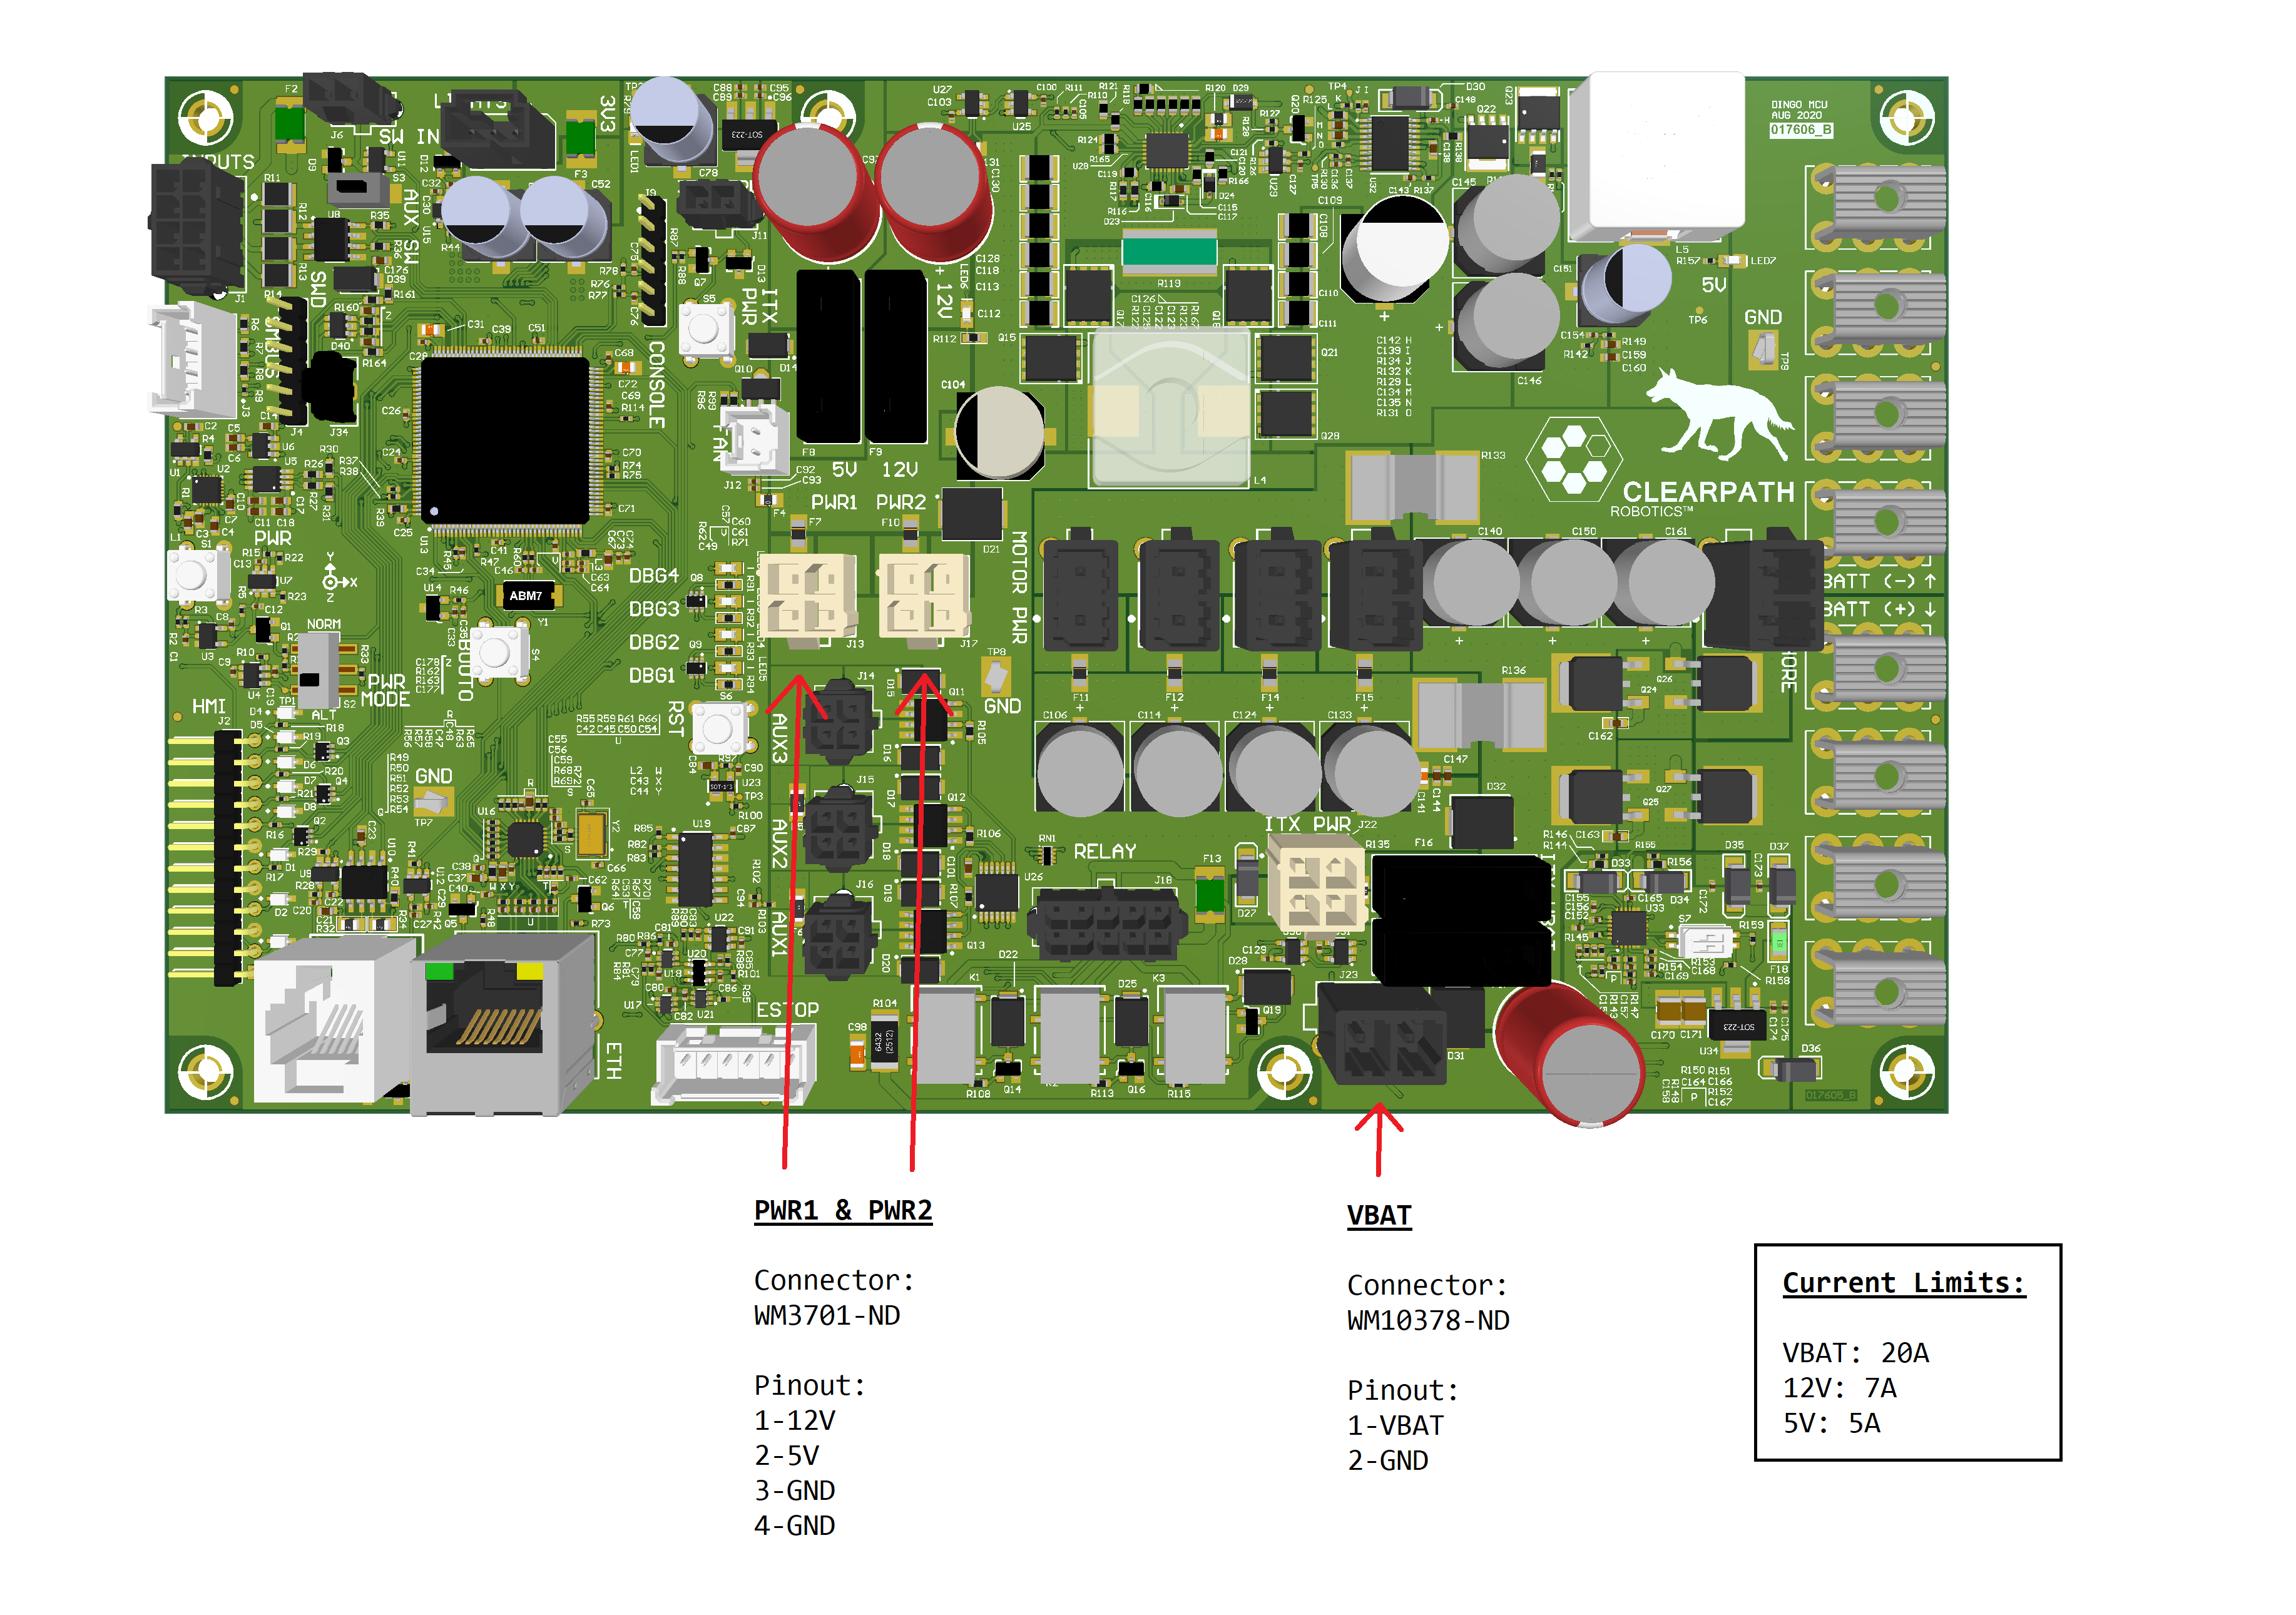
\includegraphics[width=0.9\linewidth]{dingo-mcu.png}
  \caption{Dingo MCU and User Power}
  \label{dingo-mcu}
\end{figure}

Route the power from the MCU board to the appropriate location, either to the internal payload modules or through the openings in the trough cover to the topside payload.

\subsection{Software Integration}

ROS has a large ecosystem of sensor drivers, some of which include pre-made URDF descriptions and
even simulation configurations. Please see the following page on the ROS wiki for a partial list:

\url{http://wiki.ros.org/Sensors}

For the best experience, consider purchasing supported accessories from Clearpath Robotics for your
Dingo, which will include simulation, visualization, and driver support. However, we will happily
assist you in integrating your own devices as well.


\section{Contact}\label{trouble}\label{contact}

Clearpath is committed to your success with Dingo. Please get in touch with us and we'll
do our best to get you rolling again quickly: \href{mailto:support@clearpathrobotics.com}{support@clearpathrobotics.com}

To get in touch with a salesperson regarding Dingo or other Clearpath Robotics products, please
email \href{mailto:sales@clearpathrobotics.com}{sales@clearpathrobotics.com}.

If you have a an issue that is specifically about ROS and is something which may be of interest
to the broader community, consider asking it on \href{http://answers.ros.org}{answers.ros.org}.
If you don't get a satisfactory response, please ping us and include a link to your question
as posted there. If appropriate, we'll answer in the ROS Answers context for the benefit of the
community.

Dingo is designed not to require regular maintenance. As it is a new product, Clearpath
appreciates your patience as we continue to improve the platform.

\end{document}
